%!TEX program = pdflatex
%# -*- coding: utf-8 -*-
%!TEX encoding = UTF-8 Unicode

\documentclass[12pt,oneside,a4paper]{article}

%% ------------------------------------------------------
%% load packages
\usepackage{geometry}
\geometry{verbose,tmargin=2cm,bmargin=2cm,lmargin=2cm,rmargin=2cm}
\usepackage[pdfusetitle,
 bookmarks=true,bookmarksnumbered=true,bookmarksopen=true,bookmarksopenlevel=2,
 breaklinks=false,pdfborder={0 0 1},backref=false,colorlinks=false,
 unicode=true]
 {hyperref}
\hypersetup{pdfstartview={XYZ null null 1}}
\usepackage{url}
\setcounter{secnumdepth}{2}
\setcounter{tocdepth}{2}
\usepackage{microtype}

\usepackage{amsmath, amsthm, amssymb, amsfonts}
\usepackage[retainorgcmds]{IEEEtrantools}

% \usepackage{algorithm}
% \usepackage{algorithmic}
% \renewcommand{\algorithmicrequire}{\textbf{Input:}}
% \renewcommand{\algorithmicensure}{\textbf{Output:}}
\usepackage[algoruled, vlined]{algorithm2e}

\usepackage[T1]{fontenc}
\usepackage[utf8]{inputenc}
\usepackage[mono=false]{libertine}
\usepackage[libertine]{newtxmath}
\linespread{1.05}
\setlength{\parskip}{.5\baselineskip}
% \usepackage[toc,eqno,enum,bib,lineno]{tabfigures}

\usepackage{graphics}
\usepackage{graphicx}
\usepackage[figure]{hypcap}
\usepackage[hypcap]{caption}
\usepackage{tikz}
\usepackage{tikz-cd}
%\usepackage{grffile}
%\usepackage{float}
\usepackage{pdfpages}
\usepackage{pdflscape}
\usepackage{needspace}

\usepackage{multirow}
\usepackage{booktabs}
\usepackage{threeparttable}
\usepackage{dcolumn}
\usepackage{tabu}

\usepackage{verbatim}

% \usepackage[square,numbers,super,comma,sort]{natbib}
\usepackage[backend=biber, style=nature, sorting=none, isbn=false, url=false, doi=false]{biblatex}
\addbibresource{ref.bib}
\usepackage[]{authblk}

\usepackage{etoolbox}
\BeforeBeginEnvironment{knitrout}{
    \begin{tabu} to \textwidth {XcX}
    \toprule[.7pt]
    & R Code Chunk & \\
    \bottomrule[.7pt]
    \end{tabu}
    \vspace*{-.5\baselineskip}
}
\AfterEndEnvironment{knitrout}{
    \vspace*{-.5\baselineskip}
    \noindent\rule{\textwidth}{.7pt}
}

%% Class, Exam, Date, etc.
\newcommand{\class}{STAT 5701: Statistical Computing}
\newcommand{\term}{Fall 2015}
\newcommand{\examnum}{Homework 1}
\newcommand{\hmwkTitle}{\class \\[1ex] \examnum}
\newcommand{\hmwkAuthorName}{Jingxiang Li}

\title{\hmwkTitle}
\author{\hmwkAuthorName}

\usepackage{fancyhdr}
\usepackage{extramarks}
\lhead{\hmwkAuthorName}
\chead{}
\rhead{\hmwkTitle}
\cfoot{\thepage}

\newcounter{problemCounter}
\newcounter{subproblemCounter}
\renewcommand{\thesubproblemCounter}{\alph{subproblemCounter}}
\newcommand{\problem}[0] {
    \clearpage
    \stepcounter{problemCounter}
    \setcounter{subproblemCounter}{0}
}

\newcommand{\subproblem}[0] {
    \stepcounter{subproblemCounter}
    \Needspace*{8\baselineskip}
    \vspace{1.8\baselineskip}
    \noindent{\textbf{\large{Problem \theproblemCounter.\hspace{1pt}\thesubproblemCounter}}}
    \vspace{\baselineskip}
    \newline
}

\newcommand{\solution} {
    \vspace{15pt}
    \noindent\ignorespaces\textbf{\large Solution}\par
}
\setlength\parindent{0pt}

%% some math shortcuts
\newcommand{\m}[1]{\texttt{{#1}}}
\newcommand{\E}[0]{\mathrm{E}}
\newcommand{\Var}[0]{\mathrm{Var}}
\newcommand{\sd}[0]{\mathrm{sd}}
\newcommand{\Cov}[0]{\mathrm{Cov}}
%%%%%%%%%%%%%%%%%%%%%%%%%%%%%%%%%%%%%%%%%%%%%%%%%%%%%%%%%%%%%%%%%%%%%%%%%%%

\begin{document}
\maketitle

\problem
\subproblem
The optimal $f(x)$ is $f(x) = E(y|x)$
\proof
The expected loss is
\begin{equation*}
\begin{aligned}
E_{(x,y)}[l(f(x), y)] &= \int_{x}{\int_{y}{l(f(x), y)p(y|x)dy}p(x)}dx \\
&= \int_{x}{\int_{y}{(f(x) - y)^{2}p(y|x)dy}p(x)}dx
\end{aligned}
\end{equation*}
Here we minimize the expected loss
\begin{equation*}
\min_{f}\E_{(x,y)}[l(f(x), y)] \Leftrightarrow \min_{f}\int_{y}{(f(x) - y)^{2}p(y|x)dy}
\end{equation*}
To minimize the expected loss, we take the derivative with respect to $f$, and set it to 0.
\begin{equation*}
\begin{aligned}
& \frac{\partial}{\partial f}\int_{y}{(f(x) - y)^{2}p(y|x)dy} = 0\\
\Rightarrow & \int_{y}{\frac{\partial}{\partial f}(f(x) - y)^{2}p(y|x)dy} = 0\\
\Rightarrow & \int_{y}{(f(x) - y)p(y|x)dy} = 0\\
\Rightarrow & \int_{y}{f(x)p(y|x)dy} = \int_{y}{yp(y|x)dy}\\
\Rightarrow & f(x) = E(y|x)
\end{aligned}
\end{equation*}
Q.E.D

\problem
\subproblem
\proof
The expected loss for $f$ is
\begin{equation*}
\begin{aligned}
L(f) = p(f(x) \neq y) = \E_{(x,y)}[I(f(x) \neq y)] = \int_{x}{\sum_{y}{I(f(x) \neq y)p(y|x)}p(x)}dx
\end{aligned}
\end{equation*}
Here we minimize the expected loss with respect to $f$
\begin{equation*}
\begin{aligned}
&\min_{f}\int_{x}{\sum_{y}{I(f(x) \neq y)p(y|x)}p(x)}dx \\
\Leftrightarrow &\min_{f} \sum_{y}{I(f(x) \neq y)p(y|x)}\\
\Leftrightarrow &\min_{f} I(f(x) \neq 1)p(1|x) + I(f(x) \neq -1)p(0|x)
\end{aligned}
\end{equation*}
Notice that $p(0|x) > 0$, $p(1|x) > 0$ and $p(0|x) + p(1|x) = 1$.

Considering $I(f(x) \neq 1)$ and $I(f(x) \neq 0)$, there will be exactly one has value 1, and another one 0.

Hence once $p(1|x) > p(0|x)$, the optimal $f^*$ must satisfy $f^*(x) = 1$; otherwise $f^*(x) = -1$

i.e.
\begin{equation*}
f^*(x) = \left\{ \begin{array}{ll}
+1, & \mathrm{if} ~ p(1|x) > 1/2\\
-1, & \mathrm{otherwise}
\end{array}
\right.
\end{equation*}
Since $f^*$ is optimal, $L(f^*) \leq L(f)$

Q.E.D.

\problem
\subproblem
\textbf{\em Fisher's Linear Discriminant}

Similar to Fisher's Linear Discriminant for two classes problem, we first construct the within-class covariance matrix $S_{W}$ and between class covariance matrix $S_{B}$.

Let $K$ be the number of classes, $C_k$ be the indicator of class $k$, $N_k$ be the number of observations in class $k$. Then we can derive $S_{W}$ and $S_{B}$ by:
\begin{equation*}
\begin{aligned}
    S_W &= \sum_{k = 1}^{K}{S_{k}}\\
    S_B &= \sum_{k = 1}^{K}{N_{k}(m_k - m)(m_k - m)^{T}}
    % S_{k} &= \sum_{n \in C_{k}}(x_{n} - m_{k})(x_{n} - m_{k})^T
\end{aligned}
\end{equation*}
where
\begin{equation*}
\begin{aligned}
    S_{k} &= \sum_{n \in C_{k}}(x_{n} - m_{k})(x_{n} - m_{k})^T\\
    m_{k} &= \frac{1}{N_{k}}\sum_{n\in C_{k}}{x_n}
\end{aligned}
\end{equation*}
Let $W$ be the resulting weight matrix for Fisher's Linear Discriminant, we can derive it by maximizing the following quantity
\begin{equation*}
    J(W) = \mathrm{Tr}\left\{(WS_{W}W^{T})^{-1}(WS_{B}W^{T})\right\}
\end{equation*}
The weight matrix are determined by those eigenvectors of $S_{W}^{-1}S_{B}$ that correspond to the $D'$ largest eigenvalues\cite{bishop2006pattern}.

Note that $S_{B}$ is composed from $K$ rank 1 matrices, and only $(K - 1)$ of these matrices are independent, thus $S_{B}$ has rank at most equal to (K - 1) and so there are at most (K - 1) nonzero eigenvalues. Hence we are unable to find more than $(K - 1)$ linear ``features'' by this means\cite{fukunaga1990statistical}.

Sometimes calculating eigenvectors for $S_{W}^{-1}S_{B}$ results in all complex vectors, which is due to the bad condition of $S_{W}$. For this case we simply find eigenvectors for $(S_{W} + I)^{-1}S_{B}$ as a substitute.

After obtaining the weight matrix $W$, we project $X$ by $X^{\mathrm{new}} = XW$ and treat $X^{\mathrm{new}}$ as the new design matrix for future processing.

\vspace{2em}
\textbf{\em Multivariate Gaussian Generative Model}

Multivariate Gaussian Generative Model assumes that each class of observations come from a multivariate Gaussian distribution. To make prediction for single observations, it applies the following Bayes rule
\begin{equation*}
\begin{aligned}
    p(C_{k}|x) = \frac{p(x|C_{k})p(C_{k})}{p(x)}, ~~ k = 1, \dots, K
\end{aligned}
\end{equation*}

Note that $p(x)$ is equal for all $k$, hence we can ignore the denominator of the posterior probability. To make predictions for a single observation x, we simply calculate ``prediction score'' $log(p(x|C_{k})) + log(p(C_{k}))$, which is simply the logarithm of the above formula, for all $k$ and classify it to the class with the largest ``prediction score''.

It's easy to derive $p(x|C_{k})$ and $p(C_{k})$. for $p(C_{k})$, it can be pre-specified or use the class proportion:
\begin{equation*}
    p(C_{k}) = \frac{\#\{x_{n} | x_{n} \in C_{k}\}}{\#\{x_{n}\}}
\end{equation*}

For $p(x|C_{k})$, since we assume $C_{k}$ has a multivariate normal distribution, it's sufficient to estimate the mean $\mu_{k}$ and the covariance matrix $\Cov_{k}$ of $C_{k}$, where
\begin{equation*}
\begin{aligned}
    \hat{\mu}_{k} &= \frac{1}{N_{k}}\sum_{n \in C_{k}}{x_{n}}\\
    \hat{\Cov}_{k} &= \frac{1}{N_{K} - 1}\sum_{n \in C_{k}}{(x_{n} - \hat{\mu}_{k})(x_{n} - \hat{\mu}_{k})^{T}}
\end{aligned}
\end{equation*}
Then it's straightforward to estimate $p(x|C_{k})$.

\vspace{2em}
\textbf{\em Least Squares Linear Discriminant}

Let $X \in \mathbb{R}^{n \times p}$ be the design matrix, $y \in \mathbb{R}^{n \times K}$ be the response matrix in bit-vector representation. For each class $C_{k}$, the model assumes
\begin{equation*}
    y_{i, k} = w_{k}^{T}x_{i},~~ k = 1,\dots,K
\end{equation*}
whose matrix form is
\begin{equation*}
    y = WX
\end{equation*}
To estimate $W$, we consider least square estimate, which means to minimize the following quantity
\begin{equation*}
    E_{D}(\tilde{W}) = \frac{1}{2}\mathrm{Tr}\left\{(X\tilde{W} - y)^{T}(X\tilde{W} - y)\right\}
\end{equation*}
The solution for the above optimization problem is
\begin{equation*}
    \tilde{W} = (X^{T}X)^{-1}X^{T}y
\end{equation*}
Notice that $X^{T}X$ might be invertible, in such case we use $X^{T}X + I$ as a substitute.

To make prediction for new observation $x$, we project it to $x^{T}W$ and predict it as class $k$ if the $k$th element of the resulting projected vector has the largest value among others.

\vspace{2em}
\textbf{\em Simulation Result}

The simulation is based on MNIST-1378 dataset for 4-class classification of hand written digits: 1, 3, 7 and 8. We use 10 fold cross-validation to evaluate the performance of the following two modeling procedures:

\hspace*{1em}1. Fisher's Discriminant Analysis + Multivariate Gaussian Generative Model (Fisher)\newline
\hspace*{1em}2. Least Squares Linear Discriminant (LS)

The simulation result is summarized in table \ref{fisher vs ls}. Note that they all perform well in terms of prediction, Fisher seems to be slightly better than LS method, but the difference in prediction accuracy is almost negligible.

\begin{landscape}
\begin{table}[p]
\centering
\caption{Fisher + Multivariate Gaussian V.S. Least Squares Discriminant}
\begin{tabular}{rrrrrrrrrrrrr}
\toprule
 \multicolumn{1}{c}{  } & \multicolumn{1}{c}{ Mean } & \multicolumn{1}{c}{ Std } & \multicolumn{1}{c}{ fold0 } & \multicolumn{1}{c}{ fold1 } & \multicolumn{1}{c}{ fold2 } & \multicolumn{1}{c}{ fold3 } & \multicolumn{1}{c}{ fold4 } & \multicolumn{1}{c}{ fold5 } & \multicolumn{1}{c}{ fold6 } & \multicolumn{1}{c}{ fold7 } & \multicolumn{1}{c}{ fold8 } & \multicolumn{1}{c}{ fold9 } \\
\midrule
 Fisher Train Erros & 4.66\% & 0.06\% & 4.78\% & 4.60\% & 4.61\% & 4.65\% & 4.64\% & 4.69\% & 4.74\% & 4.63\% & 4.63\% & 4.60\% \\
 LS Train Erros & 5.20\% & 0.05\% & 5.21\% & 5.17\% & 5.19\% & 5.32\% & 5.19\% & 5.21\% & 5.19\% & 5.18\% & 5.24\% & 5.15\% \\
 Fisher Test Erros & 5.37\% & 0.37\% & 5.04\% & 5.66\% & 5.53\% & 5.28\% & 5.25\% & 4.84\% & 5.18\% & 5.12\% & 5.87\% & 5.97\% \\
 LS Test Erros & 5.99\% & 0.50\% & 5.90\% & 6.38\% & 6.66\% & 4.91\% & 6.11\% & 5.83\% & 6.39\% & 5.66\% & 5.70\% & 6.32\% \\
\bottomrule
\end{tabular}
\label{fisher vs ls}
\end{table}
\end{landscape}

\problem
\subproblem
\textbf{\em Logistic Regression}

Logistic Regression assumes
\begin{equation*}
    p(C_{1}|x) = \sigma(w^{T}x)
\end{equation*}
where $\sigma(\cdot)$ is the logistic sigmoid function
\begin{equation*}
    \sigma(x) = \frac{1}{1 + \exp(-x)}
\end{equation*}
Then for a data set$\{x_{n}, y_{n}\}$, where $y_{n} \in \{0, 1\}$, the likelihood function is
\begin{equation*}
    \begin{aligned}
    p(y|x) &= \prod_{n = 1}^{N}{\sigma(w^{T}x_{n})^{y_{n}} (1 - \sigma(w^{T}x_{n}))^{1 - y_{n}}}\\
    \ln(p(y|x)) &= \sum_{n = 1}^{N}{\left\{y_{n}\ln(\sigma(w^{T}x_{n})) + (1 - y_{n})\ln(\sigma(w^{T}x_{n}))\right\}}
    \end{aligned}
\end{equation*}
To get an estimate of $w$, we maximize the regularized log likelihood function, which is equivalent to
\begin{equation*}
    \arg\min_{w} L(w) = -\ln(p(y|x)) + \frac{\lambda}{2}||w||^{2}
\end{equation*}
To solve the above optimization problem, we consider gradient descent.

It's easy to derive the first order derivative for the loss function
\begin{equation*}
    \nabla L(w) = \sum_{n = 1}^{N}(\sigma(w^{T}x_{n}) - y_{n})x_{n} + \lambda w
\end{equation*}
Then the iterative equation is
\begin{equation*}
    w := w - \alpha \nabla L(w)
\end{equation*}
where $\alpha$ is step size.

By iteratively update $w$ till convergence (or maximum number of iteration is reached), we can obtain an estimate for $w$.

\vspace{1em}
\textbf{\em Naive Bayes with Marginal Univariate Gaussian Approximation}

Naive Bayes assumes features are independent with each other, which suggests that
\begin{equation*}
    p(x_{1}, \dots, x_{p}|C_{k}) = \prod_{i = 1}^{p}{p(x_{i}|C_{k})}
\end{equation*}
By univariate Gaussian approximation, we assume each $p(x_{i}|C_{k}), ~i = 1,\dots,N , ~k = 1,\dots,K$ has a Gaussian distribution, whose parameters can be estimated from sample.

For prediction, simply apply Bayes rule
\begin{equation*}
    p(C_{k}|x) = \frac{p(x|C_{k})p(C_{k})}{p(x)} = \frac{\prod_{i = 1}^{p}{p(x_{i}|C_{k})}p(C_{k})}{p(x)}
\end{equation*}
By taking the logarithm of $p(C_{k}|x)$, we can simply derive a score for prediction
\begin{equation*}
    \mathrm{score}_{k} = \sum_{i = 1}^{p}{\log p(x_{i}|C_{k})} + \log p(C_{k})
\end{equation*}
Then we can predict new observation as class $k$ if the prediction score for class $k$ has the largest value among others.

\textbf{\em Simulation Result}

The simulation is based on Spam dataset for 2-class classification. For each iteration, we first split the whole dataset into 80\% for training and 20\% for test. Then, within training set, we randomly select 5\%, 10\%, ..., 30\% for training the classifier, and record test error for each of the inner-split. The whole procedure will be repeated 100 times. We apply this validation procedure to evaluate the prediction performance of the following two models:

\hspace*{1em}1. Logistic Regression\newline
\hspace*{1em}2. Naive Bayes with Marginal Univariate Gaussian Approximation

The simulation result is summarized in table \ref{logistic vs naive bayes} and figure \ref{fig:logistic vs naive bayes}. According to the mean test errors, Logistic Regression dominates Naive Bayes in all scenarios. As the size of training set increases, the test error of logistic regression drops significantly. However, the test error of naive Bayes seems to be insensitive to the increasing size of training set.

\begin{table}[ht!]
\centering
\caption{Logistic V.S. Naive Bayes}
\begin{tabular}{rrrrrrr}
\toprule
 \multicolumn{1}{c}{  } & \multicolumn{1}{c}{ 5 percent } & \multicolumn{1}{c}{ 10 percent } & \multicolumn{1}{c}{ 15 percent } & \multicolumn{1}{c}{ 20 percent } & \multicolumn{1}{c}{ 25 percent } & \multicolumn{1}{c}{ 30 percent } \\
\midrule
 Logistic Test Error Mean & 11.69\% & 10.04\% & 9.36\% & 8.78\% & 8.58\% & 8.38\% \\
 Logistic Test Error Std & 1.60\% & 1.15\% & 1.11\% & 1.02\% & 1.03\% & 0.95\% \\
 Naive Bayes Test Error Mean & 18.49\% & 18.33\% & 18.55\% & 18.63\% & 18.29\% & 18.66\% \\
 Naive Bayes Test Error Std & 1.86\% & 1.62\% & 1.66\% & 1.50\% & 1.43\% & 1.46\% \\
\bottomrule
\end{tabular}
\label{logistic vs naive bayes}
\end{table}

\begin{figure}[ht!]
    \centering
    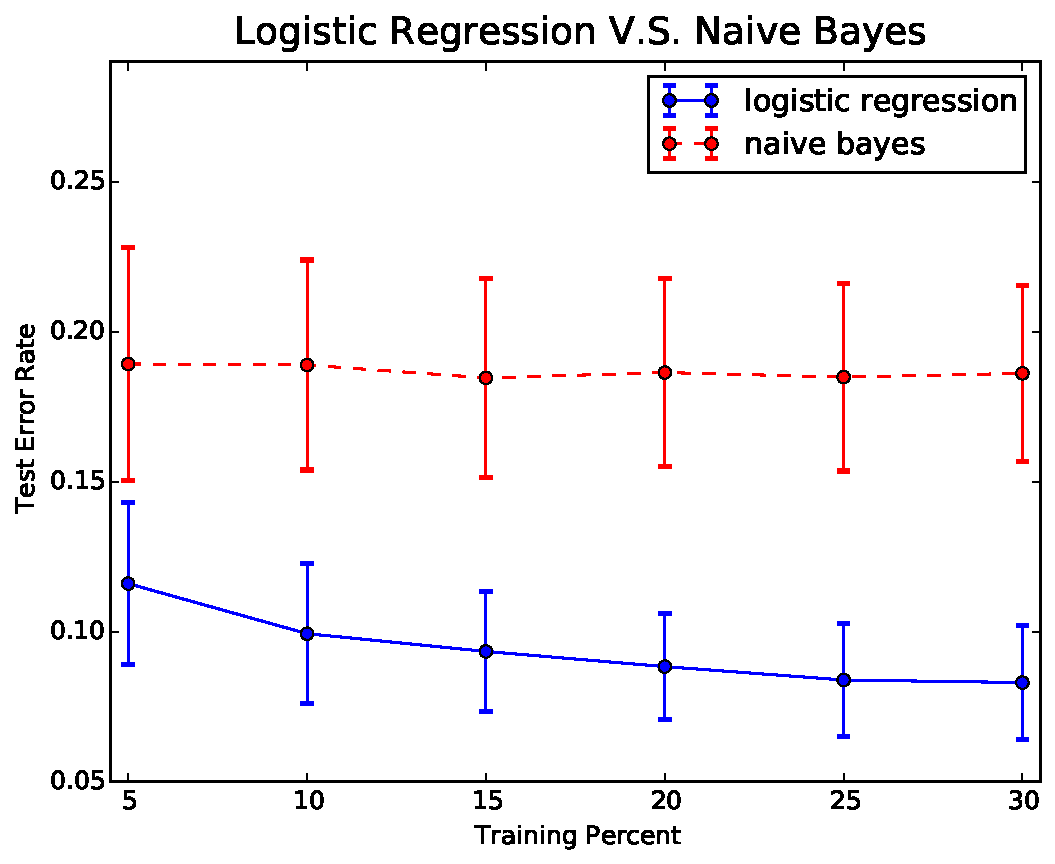
\includegraphics[width=0.6\textwidth]{./figure/nb_vs_logreg.pdf}
    \caption{Logistic V.S. Naive Bayes}
    \label{fig:logistic vs naive bayes}
\end{figure}


\clearpage
\printbibliography
\end{document}
